\chapter{Correlation and Regression}

\section*{6.1. Alternative forms of Cov(x, y) and $\bm{\widetilde{s}}$}
\addcontentsline{toc}{section}{6.1. Alternative forms of Cov(x, y) and $\widetilde{s}$}
\begin{enumerate}[(a)]
    \item Show that the Cov(x, y) defined in Eq. (6.11) can be written
        as  $\langle xy \rangle - \langle x \rangle \langle y \rangle$ 
        ($\langle x \rangle$ means the same thing as $\overline{x})$

    \item Show that the $\widetilde{s}^2$ defined in Eq. (3.60) can be
        written  as $\langle x^2 \rangle - \langle x \rangle^2$
\end{enumerate}

\vspace{1em}
\begin{proof}
    \hfill
    \begin{enumerate}[(a)]
        \item We start with Eq. (6.11) and use the average formula to obtain the desired result:
            \begin{align*}
                \text{Cov}(x, y) 
                = \frac{1}{n} \sum_{i = 1}^n (x_i - \langle x \rangle)(y_i - \langle y \rangle)
                &= \frac{1}{n} \sum_{i = 1}^n (x_iy_i - \langle x \rangle y_i - \langle y \rangle x_i +  
                    \langle x \rangle \langle y \rangle) \\
                &= \langle xy \rangle - 2 \langle x \rangle \langle y \rangle 
                    + \langle x \rangle \langle y \rangle
                = \langle xy \rangle - \langle x \rangle \langle y \rangle
            \end{align*}

        \item Similarly to (a), we start from Eq. (3.60) and find that:
            \begin{align*}
                \widetilde{s}^2 
                = \frac{1}{n} \sum_{i = 1}^n (x_i - \langle x \rangle)^2
                = \frac{1}{n} \sum_{i = 1}^n (x_i^2 - 2x_i \langle x \rangle + \langle x \rangle^2)
                = \langle x^2 \rangle - 2\langle x \rangle^2 + \langle x \rangle^2
                = \langle x^2 \rangle + \langle x \rangle^2 
            \end{align*}
    \end{enumerate}
\end{proof}

\section*{6.2. Rescaling X}
\addcontentsline{toc}{section}{6.2. Rescaling X}
Using Eq. (6.9), we showed in the third remark on page 287 that the
correlation coefficient $r$ doesn't change with a uniform scaling of
$X$ or $Y$. Demonstrate this again here by using the expression
for $r$ in Eq. (6.6).

\vspace{1em}

\begin{proof}
    Let $X' = aX$ and $Y' = bY$, where $a$ and $b$ are numerical values.
    Since $Y = mX + Z$, we notice the equivalence:
    \[
        bY = bmX + bZ \iff Y' = m'X' + cZ
    \] 
    where $m = bm/a$ and $c$ is a numerical value that we don't care about
    since the correlation coefficient $r$ does not depend on $Z$.
    From $(6.6)$ and the fact that $\text{Var}(aX) = a^2\text{Var}(X)$, we obtain:
     \[
         r' 
         = \frac{m'\sigma_{X'}}{\sigma_{Y'}} 
         = \frac{abm\sigma_{X}}{ab\sigma_{Y}}
         = \frac{m\sigma_X}{\sigma_Y} 
         = r
    \] 
    which proves once again that the correlation coefficient $r$ doesn't 
    change with a uniform scaling of $X$ or $Y$.
\end{proof}

\section*{6.3. Uncorrelated vs. independent}
\addcontentsline{toc}{section}{6.3. Uncorrelated vs. independent}
If two random variables $X$ and $Y$ are independent, are they necessarily
also uncorrelated? If they are uncorrelated, are they necessarily also independent?

\vspace{1em}

\begin{proof}
    \hfill
    \begin{enumerate}[(i)]
        \item Suppose $X$ and $Y$ are independent. We then have that $\text{Cov}(X, Y) = 0$, so,
            the correlation coefficient is given by (6.9):
            \[
                r = \frac{\text{Cov}(X, Y)}{\sigma_X\sigma_Y} = 0
            \] 
            As a result, if $X$ and $Y$ are independent, then they are also uncorrelated.

        \item We'll prove that correlation does not imply independence by giving a counterexample.
            Let $X$ be a discrete random variable with $P(X = 0) = P(X = 1) =$ 1/2 and let
            $Y = -X$. $X$ and $Y$ are independent and their covariance is given by
            \[
                \text{Cov}(X, Y) = E[XY] - \mu_X\mu_Y 
                = -E[X^2] + \frac{1}{4} 
                = -\bigg(\frac{1}{4} \cdot 1 + \frac{3}{4} \cdot 0\bigg) + \frac{1}{4}
                = 0
            \] 
            so, by (6.9), $r = 0$. Therefore, two random variables can be uncorrelated
            without being necessarily independent.
    \end{enumerate}
\end{proof}

\section*{6.4. Sum of two Gaussians (TO DO: PDF of sum)}
\addcontentsline{toc}{section}{6.4. Sum of two Gaussians}
Given two independent Gaussian distributions $X$ and $Y$ with
standard deviations $\sigma_X$ and $\sigma_Y$, show that the sum
$Z \equiv X + Y$ is a Gaussian distribution with standard
deviation $\sqrt{\sigma_X^2 + \sigma_Y^2}$. You may assume without
loss of generality that the means are zero.

\vspace{1em}

\begin{proof}
    We start by seeing that
    \[
        \mu_Z = E[Z] = E[X + Y] = \mu_X + \mu_Y
    \] 

    Now, by using the variance formula
    \[
        \sigma_Z^2 = E[Z^2] - \mu_Z^2 
        = E[(X+Y)^2] - \mu_Z^2
        = E[X^2 + 2XY + Y^2] - \mu_Z^2
    \] 

    By using the linearity of expectation and then the fact that $X$ and $Y$ are
    independent, our expression becomes:
     \[
         \sigma_Z^2 
         = E[X^2] + 2E[X]E[Y] + E[Y^2] - \mu_Z^2
         = E[X^2] + 2\mu_X\mu_Y + E[Y^2] - \mu_Z^2
    \] 

    We expand $\mu_Z^2$ and notice the expressions of $\sigma_X^2$ and $\sigma_Y^2$:
     \[
         \sigma_Z^2 = E[X^2] - \mu_X^2 + E[Y^2] - \mu_Y^2 = \sigma_X^2 + \sigma_Y^2
    \] 

    Finally, we take the square root of the variance to get the standard deviation:
    \[
        \sigma_Z = \sqrt{\sigma_X^2 + \sigma_Y^2}
    \] 
\end{proof}

\section*{6.5. Maximum $\bm{\rho(x, y)}$}
\addcontentsline{toc}{section}{6.5. Maximum $\rho(x, y)$}
For a given $y_0$, what value of $x$ maximizes the probability density
$\rho(x, y_0)$ in Eq. (6.34)?

\vspace{1em}

\begin{proof}
    The joint probability density $\rho(x, y_0)$ is given by
    \begin{equation*}\tag{6.34}
        \rho(x, y) = \frac{1}{2\pi\sigma_X\sigma_Y\sqrt{1 - r^2}} 
        \exp\bigg(-\frac{1}{2(1 - r^2)}\bigg(\frac{x^2}{\sigma_X^2} 
            + \frac{y_0^2}{\sigma_Y^2} - \frac{2rxy_0}{\sigma_X\sigma_Y}\bigg)\bigg)
    \end{equation*}

    Let
    \[
        \phi(x) 
        = \bigg(\frac{x^2}{\sigma_X^2} + \frac{y_0^2}{\sigma_Y^2} - \frac{2rxy_0}{\sigma_X\sigma_Y}\bigg) 
    \] 

    We notice that $x$ is used only in the second factor of the exponential, so
    $\rho(x, y_0)$ is maximised when $\phi(x)$ is minimised (there is a "-" sign in the exponential). We take the derivative of $\phi(x)$
    with respect to $x$ and  obtain
    \[
        \pdv{x} \phi(x) 
        = \pdv{x} \bigg(\frac{x^2}{\sigma_X^2} + \frac{y_0^2}{\sigma_Y^2} - \frac{2rxy_0}{\sigma_X\sigma_Y}\bigg) 
        = \frac{2x}{\sigma_X^2} - \frac{2ry_0}{\sigma_X\sigma_Y}
        = \frac{2x\sigma_Y - 2ry_0\sigma_X}{\sigma_X^2\sigma_Y}
    \] 

    If we equalize the derivative with 0, we obtain the critical point
    \[
        x_0 = ry_0 \frac{\sigma_X}{\sigma_Y}
    \] 

    Since the derivative is negative on the left of $x_0$ and positive on the right of $x_0$,
    we get that $x_0$ is the global minimum of $\phi(x)$. As a result, $x_0$ is the global maximum
    of $\rho(x, y_0)$.
\end{proof}

\section*{6.8. Alternate form of B}
\addcontentsline{toc}{section}{6.8. Alternate form of B}
Show that the second expression for $B$ in Eq. (6.49) equals
the first.

\vspace{1em}

\begin{proof}
    \begin{align*}\tag{6.49}
        \langle y \rangle - A \langle x \rangle 
        = \langle y \rangle - \langle x \rangle 
        \frac{\langle xy \rangle - \langle x \rangle \langle y \rangle}{\langle x^2 \rangle - \langle x \rangle^2}
        &= \frac{\langle y \rangle \langle x^2 \rangle - \langle y \rangle \langle x \rangle^2
            - \langle x \rangle \langle xy \rangle - \langle x \rangle^2 \langle y \rangle}
            {\langle x^2 \rangle - \langle x \rangle^2} \\
        &= \frac{\langle y \rangle \langle x^2 \rangle - \langle x \rangle \langle xy \rangle}
            {\langle x^2 \rangle - \langle x \rangle^2}
        = B
    \end{align*}
\end{proof}

\section*{6.9. Finding all the quantities}
\addcontentsline{toc}{section}{6.9. Finding all the quantities}
Given five ($X, Y$) points with values (2, 1), (3, 1), (3, 3),
(5, 4), (7, 6), calculate (with a calculator) all of the quantities
reffered to in the five steps listed on page 290. Also calculate
$B$ in Eq. (6.49), and make a rough plot of the five given points
along with the regression (least-squares) line.

\vspace{1em}

\begin{proof}
    \hfill
    \begin{enumerate}[1.]
        \item Compute the means $\overline{x}$ and $\overline{y}$ of the $x_i$ and 
             $y_i$ data points:
             \[
                 \overline{x} = \frac{2 + 3 + 3 + 5 + 7}{5} = 4
                 \hspace{2em}
                 \overline{y} = \frac{1 + 1 + 3 + 4 + 6}{5} = 3
             \] 

         \item Calculate the standard deviations $\widetilde{s_x}$ and $\widetilde{s_y}$ via 
             Eq. (3.60):
             \begin{align*}
                 \widetilde{s_x} = \sqrt{\frac{(2 - 4)^2 + (3 - 4)^2 + (3 - 4)^2 + (5 - 4)^2 + (7 - 4)^2}{5}} 
                    = \frac{4}{\sqrt{5}} \approx 1.79 \\
                \widetilde{s_y} = \sqrt{\frac{(1 - 3)^2 + (1 - 3)^2 + (3 - 3)^2 + (4 - 3)^2 + (6 - 3)^2}{5}}
                    = 3 \sqrt{\frac{2}{5}} \approx 1.9
             \end{align*}
            
        \item Calculate the covariance via Eq. (6.11):
            \begin{align*}
                \text{Cov}(x, y) 
                &= \frac{(2 - 4)(1 - 3) + (3 - 4)(1 - 3) + 
                    (3 - 4)(3 - 3) + (5 - 4)(4 - 3) + (7 - 4)(6 - 3)}{5} \\
                &= \frac{16}{5} = 3.2
            \end{align*}

        \item Calculate $r$ via Eq. (6.12):
            \[
                r = \frac{\text{Cov}(x, y)}{\widetilde{s_x}\widetilde{s_y}}
                = \frac{3.2}{1.79 \cdot 1.9} \approx 0.94
            \] 

        \item Calculate $m$ from Eq. (6.18), with the $\sigma$'s replaced with $\widetilde{s}$'s :
            \[
                m = \frac{r\widetilde{s_y}}{\widetilde{s_x}} 
                = \frac{0.94 \cdot 1.9}{1.79} \approx 1
            \] 
        \end{enumerate}
        \begin{figure}[H]     
        \center{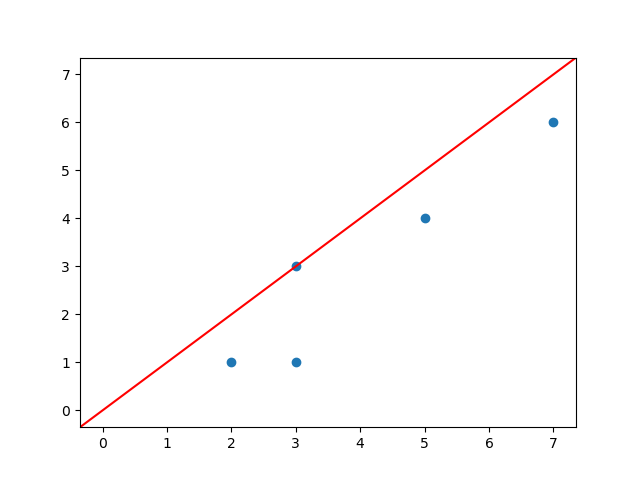
\includegraphics[width=0.50\linewidth]{figure_6_9.png}}
        \end{figure}
\end{proof}

\section*{6.10. Equal distances}
\addcontentsline{toc}{section}{6.10. Equal distances}
In Section 6.9. we defined the best-fit line as the line that minimizes
the sum of the squares of the vertical distance from the given point
to the line. Let's kick things down a dimension and look at the 1-D
case where we have $n$ values $x_i$ lying on the $x$ axis. We'll define
the "best-fit" point as the value of $x$ (call it $x_b$) that minimizes 
the sum of the squares of the distances from the  $n$ given $x_i$ points
to the $x_b$ point.

\begin{enumerate}[(a)]
    \item Show that $x_b$ is the mean of the $x_i$ values.
    
    \item Show that the sum of all the distances from $x_b$ to the
        points with $x_i > x_b$ equals the sum of all the distances
        from $x_b$ to the points with $x_i < x_b$.
\end{enumerate}

\vspace{1em}

\begin{proof}
    \hfill
    \begin{enumerate}[(a)]
        \item Let us define
            \[
                S \equiv \frac{1}{n} \sum_{i = 1}^n (x_i - x_b)^2
            \] 
            
        The value for $x_b$ for which $S$ is minimized can be found between the values
        for which the derivative of $S$ with respect to $x_b$ is 0. We have that:
        \[
            \pdv{x_b}S = \frac{1}{n} \sum_{i = 1}^n \pdv{x_b}(x_i^2 - 2x_i x_b + x_b^2) 
            = \frac{1}{n} \sum_{i = 1}^n (2x_b - 2x_i) = 2x_b - \frac{2}{n} \sum_{i = 1}^n x_i
            = 2x_b - 2\overline{x}
        \] 

        Therefore, $x_b = \overline{x}$ is a critical point for $S$. Since the slope
        of $S$ is positive and then negative around $x_b$, we obtain that $x_b = \overline{x}$
        is an absolute minimum point for $S$. 

    \item We can assume without loss of generality that the points are labeled such that
        for $i \leq M$, $x_i < x_b$ and for $i > M, x_i > x_b$. Hence, there are $M$ points
        that are less than $x_b$ and $(n - M)$ points that are greater than $x_b$. Our
        hypothesis becomes equivalent with the expression 
        \[
            \sum_{i = 1}^M (x_b - x_i) = \sum_{i = M + 1}^n (x_i - x_b)
        \] 
        We separate the $x_b$ terms from the sums and obtain that
        \[
            Mx_b - \sum_{i = 1}^M x_i = (M - n) x_b + \sum_{i = M + 1}^n x_i
        \] 

        If we isolate the $x_b$ from the sum terms, we have that
        \[
            nx_b = \sum_{i = 1}^{n} x_i
        \] 

        which with $x_b = \overline{x}$, the result that we proved at (a). Therefore,
        we proved the hypothesis.
    \end{enumerate}
\end{proof}

\section*{6.11. Equal distances again}
\addcontentsline{toc}{section}{6.11. Equal distances again}
Returning to 2-D, show that the sum of all the vertical distances from 
the least-squares line to the points above it equals the sum of all the vertical
distances from the line to the points below it. $\emph{Hint:}$ Consider an appropriate
partial derivative of the sum $S$ in Eq. (6.42).

\vspace{1em}

\begin{proof}
    The solution is similar to 6.10b. We assume without loss of generality that 
    the $n$ points are labeled such that for $i \leq M$,
    $y_i < Ax_i + B$ and  for $i > M, y_i > Ax_i + B$. Hence, there are $M$ 
    points that are under the least-squares line and $(n - M)$ above it. 
    Our hypothesis becomes equivalent with the expression
    \[
        \sum_{i = 1}^M (Ax_i + B - y_i) = \sum_{i = M + 1}^n (y_i - Ax_i + B)
    \] 
    We expand the sum to obtain that
    \[
        A \sum_{i = 1}^M x_i + BM - \sum_{i = 1}^M y_i 
        = \sum_{i = M + 1}^n y_i - A\sum_{i = M + 1}^n x_i + (n - M)B
    \] 
    We separate the $B$ terms from the rest of the expression and get that
    \[
        nB = \sum_{i = 1}^n y_i - A\sum_{i = 1}^n x_i 
    \] 
    which if we divide by $n$ and rewrite using the average operator, is equivalent with
    \begin{equation}\tag{6.49}
        B = \langle y \rangle - A \langle x \rangle
    \end{equation}
    which we know it's true. Therefore, we proved our hypothesis.
\end{proof}
